
Найдём распределение случайной величины $\nu$:

\begin{sympycode}
n = symbols("n")
nu1 = nu.subs(eta, y)
supp_nu = ImageSet(Lambda(y, nu1), y_interval)
supp_nu1 = FiniteSet(1,2,3,4,5)
\end{sympycode}

Носитель случайной величины $\nu$:
\[
    \supp \nu = \sympy{supp_nu} = \sympy{supp_nu1}
\]

\begin{figure}[h!]
    \centering
    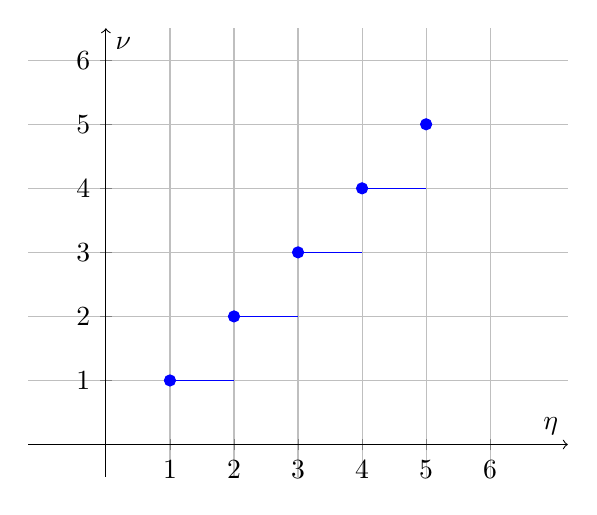
\begin{tikzpicture}
        \begin{axis}[
                xlabel=$\eta$,
                ylabel=$\nu$,
                xmin=-0.5, xmax=6.5,
                ymin=-0.5, ymax=6.5,
                axis lines=middle,
                axis line style={->},
                yscale=1,
                xscale=1,
                % ticks=none,
                % clip=true,
                xtick={0, 1, 2, 3, 4, 5, 6},
                ytick={0, 1, 2, 3, 4, 5, 6},
                grid=both,
                axis equal,
            ]
            \addplot[domain=1:5, blue, solid] (1,1) -- (2,1);
            \addplot[mark=*, mark size=2pt, blue] coordinates {(1,1)};
            \addplot[domain=1:5, blue, solid] (2,2) -- (3,2);
            \addplot[mark=*, mark size=2pt, blue] coordinates {(2,2)};
            \addplot[domain=1:5, blue, solid] (3,3) -- (4,3);
            \addplot[mark=*, mark size=2pt, blue] coordinates {(3,3)};
            \addplot[domain=1:5, blue, solid] (4,4) -- (5,4);
            \addplot[mark=*, mark size=2pt, blue] coordinates {(4,4)};

            \addplot[mark=*, mark size=2pt, blue] coordinates {(5,5)};

        \end{axis}
    \end{tikzpicture}
    \caption{График величины $\nu$ в зависимости от $\eta$}
    \label{fig:nu}
\end{figure}

\begin{sympycode}
y_by_t1 = Interval(1,2)
y_by_t2 = Interval(2,3)
y_by_t3 = Interval(3,4)
y_by_t4 = Interval(4,5)
y_by_t5 = 5
p_nu1 = integrate(p_eta, (y, y_by_t1.start, y_by_t1.end))
p_nu2 = integrate(p_eta, (y, y_by_t2.start, y_by_t2.end))
p_nu3 = integrate(p_eta, (y, y_by_t3.start, y_by_t3.end))
p_nu4 = integrate(p_eta, (y, y_by_t4.start, y_by_t4.end))
p_nu5 = integrate(p_eta, (y, y_by_t5, y_by_t5))
\end{sympycode}

Величина $\nu$ дискретная. Поэтому для каждого значения $\nu$ найдём вероятность. Для этого разобьём носитель $\eta$ на отрезки.

1) $\nu = 1 \Rightarrow \eta \in \sympy{y_by_t1}$
\[
    A_1 = \sympy{y_by_t1} \Rightarrow
    {p_\nu}_1
    = \int\limits_{\sympy{y_by_t1.start}}^{\sympy{y_by_t1.end}} p_{\eta} (y) \, dy
    = \int\limits_{\sympy{y_by_t1.start}}^{\sympy{y_by_t1.end}} \sympy{p_eta} \, dy
    = \sympy{p_nu1}.
\]

2) $\nu = 2 \Rightarrow \eta \in \sympy{y_by_t2}$
\[
    A_2 = \sympy{y_by_t2} \Rightarrow
    {p_\nu}_2
    = \int\limits_{\sympy{y_by_t2.start}}^{\sympy{y_by_t2.end}} p_{\eta} (y) \, dy
    = \int\limits_{\sympy{y_by_t2.start}}^{\sympy{y_by_t2.end}} \sympy{p_eta} \, dy
    = \sympy{p_nu2}.
\]

3) $\nu = 3 \Rightarrow \eta \in \sympy{y_by_t3}$
\[
    A_3 = \sympy{y_by_t3} \Rightarrow
    {p_\nu}_3
    = \int\limits_{\sympy{y_by_t3.start}}^{\sympy{y_by_t3.end}} p_{\eta} (y) \, dy
    = \int\limits_{\sympy{y_by_t3.start}}^{\sympy{y_by_t3.end}} \sympy{p_eta} \, dy
    = \sympy{p_nu3}.
\]
4) $\nu = 4 \Rightarrow \eta \in \sympy{y_by_t4}$
\[
    A_4 = \sympy{y_by_t4} \Rightarrow
    {p_\nu}_4
    = \int\limits_{\sympy{y_by_t4.start}}^{\sympy{y_by_t4.end}} p_{\eta} (y) \, dy
    = \int\limits_{\sympy{y_by_t4.start}}^{\sympy{y_by_t4.end}} \sympy{p_eta} \, dy
    = \sympy{p_nu4}.
\]
5) $\nu = 5 \Rightarrow \eta \in \sympy{y_by_t5}$
\[
    A_5 = \sympy{y_by_t5} \Rightarrow
    {p_\nu}_5
    = \int\limits_{\sympy{y_by_t5}}^{\sympy{y_by_t5}} p_{\eta} (y) \, dy
    = \int\limits_{\sympy{y_by_t5}}^{\sympy{y_by_t5}} \sympy{p_eta} \, dy
    = \sympy{p_nu5}.
\]

Итого, вероятность получить каждое из значений случайной величины $\nu$:
\begin{sympycode}
p_nu = Piecewise((p_nu1, Eq(n, 1)), (p_nu2, Eq(n, 2)), (p_nu3, Eq(n, 3)), (p_nu4, Eq(n, 4)), (p_nu5, Eq(n, 5)), (0, True))
\end{sympycode}
\begin{table}[h!]
    \centering
    \caption{Распределение случайной величины $\nu$}
    \begin{tabular}{|c|c|c|c|c|c|}
        \hline
        $\nu$   & 1               & 2               & 3               & 4               & $\sum$ \\
        \hline
        $\Prob$ & $\sympy{p_nu1}$ & $\sympy{p_nu2}$ & $\sympy{p_nu3}$ & $\sympy{p_nu4}$ & 1      \\
        \hline
    \end{tabular}
\end{table}

Найдём мат. ожидание и дисперсию случайной величины $\nu$:

\begin{sympycode}
Expect_nu = Sum(n * p_nu, (n, 1, 4))
Expect_nu1 = Expect_nu.doit()
Expect_nu_square = Sum(n ** 2 * p_nu, (n, 1, 4)).doit()
Variance_nu1 = Expect_nu_square - Expect_nu1 ** 2
\end{sympycode}
\[
    \begin{aligned}
        \Expect\nu
         & = \sum\limits_{n=1}^{4} n \cdot p_\nu (n)
        = \sympy{Expect_nu1},                         \\
        \Variance\nu
         & = \Expect\nu^2 - \left(\Expect\nu\right)^2
        = \sum\limits_{n=1}^{4} n^2 \cdot p_\nu (n) - \left(\Expect\nu\right)^2
        = \sympy{Expect_nu_square} - \left(\sympy{Expect_nu1}\right)^2
        = \sympy{Variance_nu1}.
    \end{aligned}
\]

Построим графики функций распределения $F_\nu(n)$:

\begin{sympycode}
F_nu1 = Piecewise(
    (0, n <= 1),
    (Sum(p_nu, (n, 1, 1)).doit(), n <= 2),
    (Sum(p_nu, (n, 1, 2)).doit(), n <= 3),
    (Sum(p_nu, (n, 1, 3)).doit(), n <= 4),
    (Sum(p_nu, (n, 1, 4)).doit(), n <= 5),
    (1, True)
)
F_nu1 = piecewise_exclusive(piecewise_fold(F_nu1))
\end{sympycode}

\[
    F_\nu (n) = \sum\limits_{x=1}^{n} p_\nu (x)
\]

\[
    F_\nu (n) = \sympy{F_nu1}
\]

\begin{figure}
    \centering
    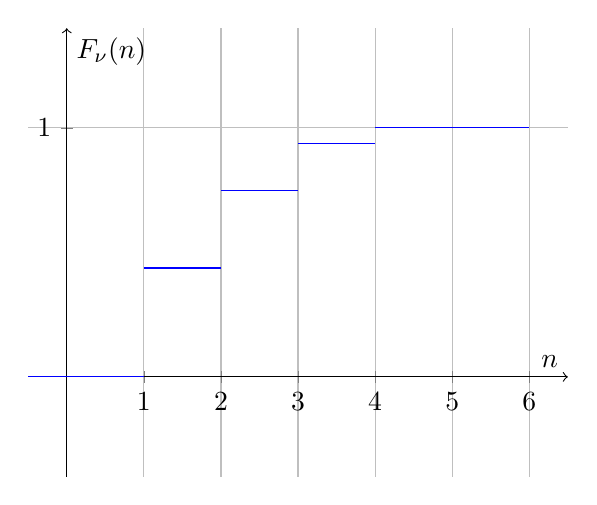
\begin{tikzpicture}
        \begin{axis}[
                xlabel=$n$,
                ylabel=$F_\nu(n)$,
                xmin=-0.5, xmax=6.5,
                ymin=-0.4, ymax=1.4,
                axis lines=middle,
                axis line style={->},
                % yscale=1,
                % xscale=1,
                % ticks=none,
                % clip=true,
                xtick={0, 1, 2, 3, 4, 5, 6},
                ytick={0, 1},
                grid=both,
            ]
            \addplot[domain=1:5, blue, solid] (-1,0) -- (1,0);
            \addplot[domain=1:5, blue, solid] (1,7/16) -- (2,7/16);
            \addplot[domain=1:5, blue, solid] (2,0.75) -- (3,0.75);
            \addplot[domain=1:5, blue, solid] (3,15/16) -- (4,15/16);
            \addplot[domain=1:5, blue, solid] (4,1) -- (6,1);

        \end{axis}
    \end{tikzpicture}
    \caption{График функции распределения $F_\nu(n)$}
    \label{fig:F_nu}
\end{figure}